\documentclass{article}
\usepackage[margin=1.0in]{geometry}
\usepackage{longtable}

\usepackage{amsmath}

\newcounter{example}
\newenvironment{example}[1][]{\refstepcounter{example}\par\medskip
   \noindent \textit{Example~\theexample. #1} \rmfamily}{\medskip}

\usepackage{bbm}
\usepackage{booktabs}

\newcommand{\fabs}[1]{\mid {#1} \mid}
\usepackage{hyperref}

\newcommand{\bet}[1]{\llbracket {#1} \rrbracket^{\beta} }
\usepackage{stmaryrd}
\usepackage{graphicx}
\usepackage{tikz}
\usepackage{wrapfig}
\usepackage{makecell}

% \usepackage{mathabx}
\usepackage{amssymb,forest}

\usepackage{float}
\usepackage{MnSymbol}
\newlength\q
\newlength\smallCol
\newlength\argsLen
\setlength\q{\dimexpr .5\textwidth -2\tabcolsep}
\setlength\smallCol{\dimexpr .15\textwidth}
\setlength\argsLen{\dimexpr .2\textwidth}


\newcommand{\lto}{\mathbin{\to}}
\usepackage{booktabs}
\usepackage{enumitem} 
\usepackage{array}% for extended column definitions
\usepackage{graphicx}
\usepackage{verbatim}
\usepackage{tabto}
\newcommand{\ov}[2]{\ensuremath{\overset{\cdot {#2} \cdot}{#1}}}
\newcommand{\imp}{\rightarrow}

\usepackage{xstring}
\usepackage[german]{babel}
\usepackage[utf8]{inputenc}

\usepackage{lipsum}
\usepackage{listings}
\usepackage{color}

\definecolor{dkgreen}{rgb}{0,0.6,0}
\definecolor{gray}{rgb}{0.5,0.5,0.5}
\definecolor{mauve}{rgb}{0.58,0,0.82}

\lstset{frame=tb,
  language=Java,
  aboveskip=3mm,
  belowskip=3mm,
  showstringspaces=false,
  columns=flexible,
  basicstyle={\small\ttfamily},
  numbers=none,
  numberstyle=\tiny\color{gray},
  keywordstyle=\color{blue},
  commentstyle=\color{dkgreen},
  stringstyle=\color{mauve},
  breaklines=true,
  breakatwhitespace=true,
  tabsize=3
}
\lstset{language=Python}

\title{Gralog External Programming Manual}

\author{Felix Herron\\\texttt{felix.herron@tu-berlin.de} \and Roman
  Rabinovich\\ \texttt{roman.rabinovich@tu-berlin.de}}

\date{August 2018}

\begin{document}

\maketitle


\begin{abstract}
Gralog is a visual tool for working with graphs, logics, games,
transition systems and other structures based on undirected and
directed graphs. It can create, load, save and edit graphs in
various formats.

The key focus of Gralog is simplicity of use and a short time of
learning how to use it.

A special property of Gralog is that it helps the developer to write
programmes for graphs in any language capable of working with
pipes. Gralog visualises the run of the programme and can keep track
of values of user defined variables.

The interaction between Gralog and the external programme is
performed by a simple, but powerful protocol. In the first version
we implemented a library for Python that simplifies the interaction
and abstracts away the use of pipes. This paper describes the
protocol and the library, the External Programming Module (EPM). This
includes documentation of methods and classes pertaining to the
EPM and code examples for how to use these.
\end{abstract}

\section{Documentation and Installation}

You can download Gralog from \url{www.gralog.org} (Change this)

Gralog is written in Java and does not need special installation. Just
run the jar file by

[code, including where the jar file is]

or run Gralog directly from the source code by calling

[code: ./gradlew].

The documentation can be found in directory \texttt{doc/}. The main
manual file is \texttt{gralog.pdf}. This part is additionally in the
file \texttt{external.pdf}. [TODO: make a general manual, include this
text there.]



\section{Setting up your External Python Programme}
To link your script to Gralog, locate the Gralog folder in your
Terminal. Navigate to the \emph{scripts} directory with gralog-fx piping
subdirectory. That should entail something like:
\begin{align*}
&\text{~/path.to.gralog/gralog/gralog-fx/src/main/java/gralog/gralogfx/piping/scripts}
\end{align*}

Once there, you will find a file called Lib.py. This is the library that defines the interactions with Gralog.\\

Now create a new file in the directory, called HelloWorld.py. In the document, paste the following code: 

\begin{lstlisting}
#!/usr/bin/python
#HelloWorld.py
from Lib import *
#A simple Gralog program which creates a vertex that says "Hello, world"

g = Graph(None); #uses the current graph that is open
v = g.addVertex();
v.setLabel("Hello, world!");
\end{lstlisting}

Now before you can run this code, open Gralog and select Preferences from the File menu. Navigate to General, then select the file you created at \emph{Ext. Prog. Source File}. Click \textbf{``Ok''.}

Now you should be ready to run. Navigate to File Menu and select "Load Plugin". What you should get is something that looks like this: 

\begin{figure}[H]
\centering
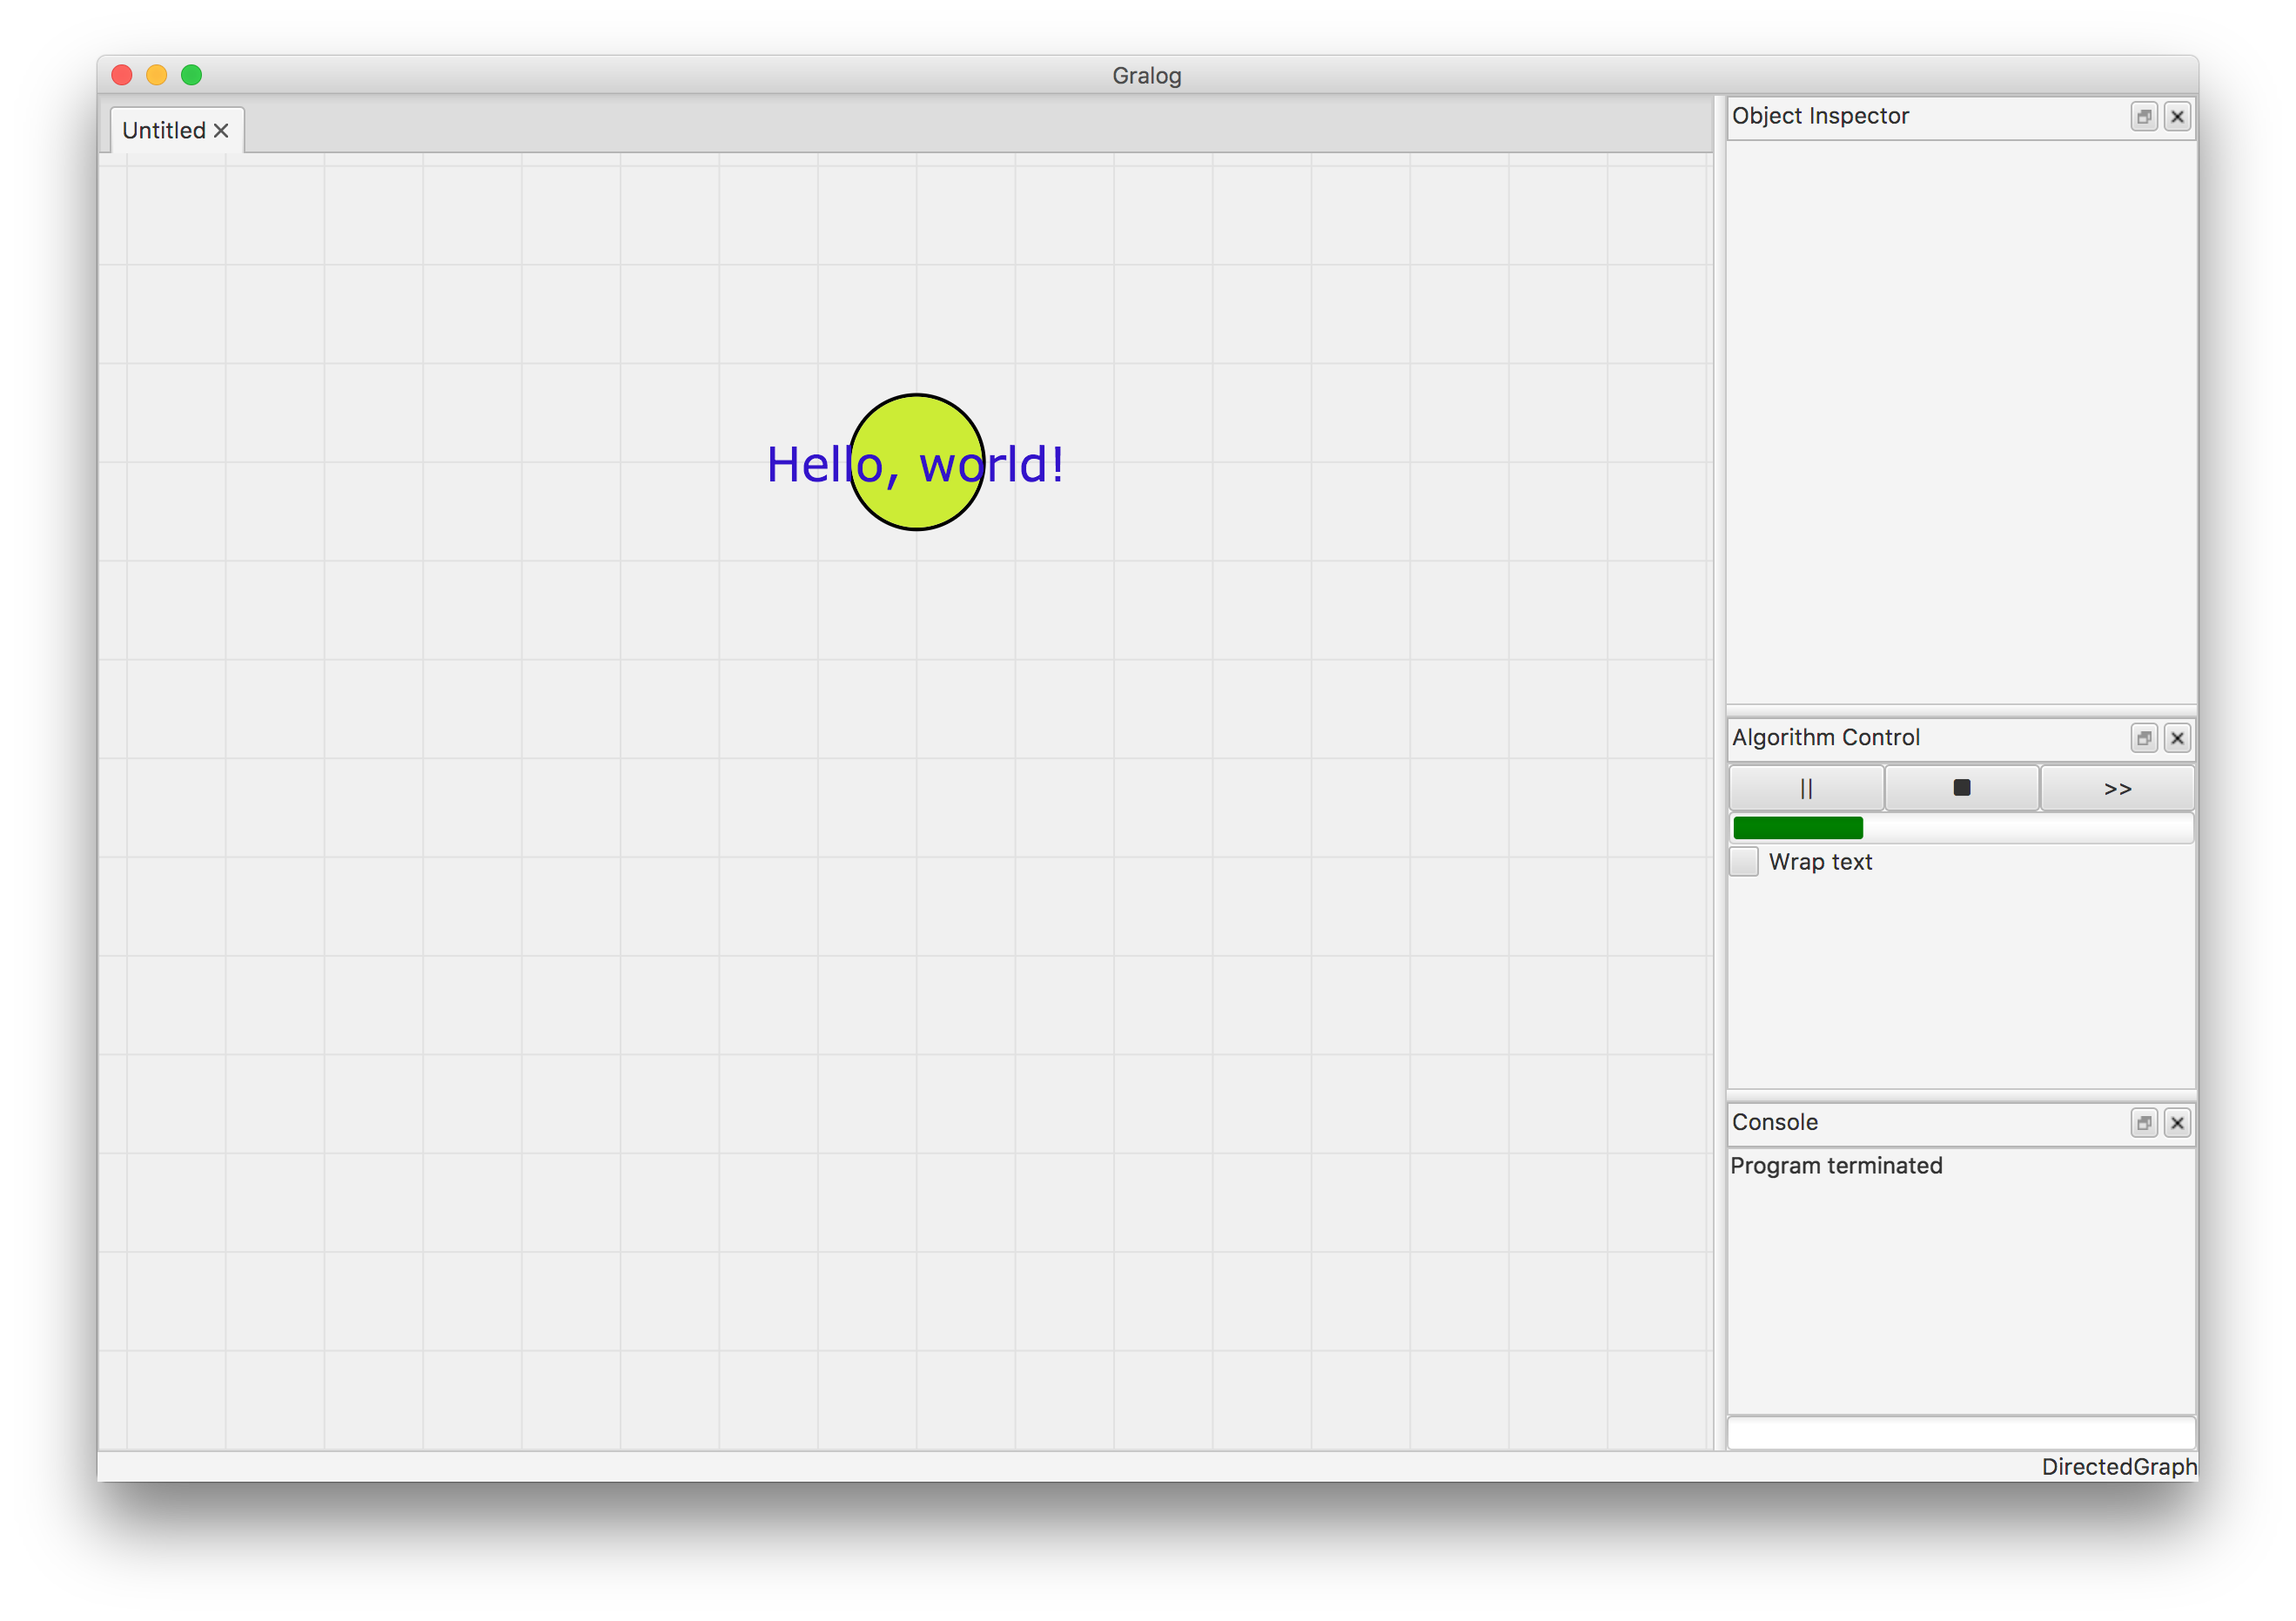
\includegraphics[width=\textwidth]{helloWorld.png}
\end{figure}

\subsection{Troubleshooting}
First obviously make sure you have python installed (version $\ge
2.7$). Also make sure that Lib.py is in the directory as the file you
wish to execute. Obviously you can mess around with the file structure
to fit your needs but in this configuration they must be in the same
directory. For other outstanding problems feel free to shoot an email
at \texttt{gralog@tu-berlin.de} (TODO: make the email address.)

\section{Introduction}
Now that you have the code running and set up, what will follow is a brief explanation of all of the functionality which we have built, structured in an intuitive manner.

\subsection{The Graph Class}
The first relevant class is Graph. In every program, you must choose a graph on which to execute your program. This is accomplished by instantiating the class Graph. 

\begin{lstlisting}
g = Graph();
\end{lstlisting}

In the constructor you specify which type of graph (directed,
undirected, a Kripke structure, a finite automaton, a Büchi automaton) you would like. No
argument means use the graph that is currently opened in Gralog, whatever (type) it may be.

The Graph class can be seen as the moderator of the program. You will use it to do all of the surface-level, more general commands pertaining to the graph itself. The more intricate details will be done using the following two:

\subsection{The Vertex Class}
Each vertex is represented as an object of the class Vertex. It is distinguished by its unique ID. 

\begin{lstlisting}
v = g.createVertex();
\end{lstlisting}

All methods pertaining to the individual vertices, such as their color, neighbours, or label, are most easily manipulated using methods of this class. For example:

\begin{lstlisting}
v = g.createVertex(id=42);
v.setLabel("f00");
neighbours = v.getNeighbours();
myLabel = v.getLabel();
v.delete();
\end{lstlisting}

\subsection{The Edge Class}
Each edge is represented as an object of hte Edge class. It is distinguished by its unique ID; however, in graphs without multi-edges, it can also be distinguished by its source and target vertices.

\begin{lstlisting}
e = g.createEdge(v1, v2, directed=False);
\end{lstlisting}

All methods pertaining to the individual edges, such as their color, adjacent edges, or label, are most easily manipulated using methods of this class. For example:

\begin{lstlisting}
e = g.createEdge(v1, v2, directed=False, id=451);
e.setLabel("f00");
adjacentEdges = e.getAdjacentEdges();
target = e.getTarget();
e.delete();
\end{lstlisting}

The documentation will now simply elaborate on these concepts.

\section{Documentation}

\subsection{Class Graph}

\textbf{{\large Instance Variables}}


\begin{longtable}{p{\q}p{\q}}
Instance Variable & Meaning and Usage \\ \hline
\textbf{Dictionary} \textit{vertices} & A dictionary that holds all of the Vertex objects known to the graph. This should ideally not be changed by the programmer. \\\hline
\textbf{Dictionary} \textit{edges} & A dictionary that holds all of the Edge objects known to the graph. This should ideally not be changed by the programmer. \\\hline
\textbf{Integer} \textit{id} & The id of the graph that is used in communication with gralog. This should ideally not be changed by the programmer. \\ \hline
\textbf{Dictionary} \textit{variablesToTrack} & Objects in format (name,value). These are displayed in the Algorithm Control Panel. These may be changed. \\ \hline
\textbf{Dictionary} \textit{variablesToTrack} & Objects in format (name,value). These are displayed in the Algorithm Control Panel. These may be changed. \\ \hline
\end{longtable}


\textbf{{\large Relevant Methods}}
\textit{Note: optional parameters are in square brackets}


\begin{description}
\item[Graph({[str: format]})] \emph{returns} a Graph Object.


                                               The graph is the graph
currently opened in the Gralog tab from which your script has been
called. (TODO: finish description) Possible parameter options are:
\begin{itemize}
\item nothing, e.g.\@ \texttt{g = Graph()},
\item \texttt{"directed"},
\item \texttt{"{}undirected"},
\item \texttt{"buechi"},
\item \texttt{"kripke"},
\item \texttt{"{}automaton"}.
\end{itemize}
\end{description}

\subsection{Graph Manipulating Methods}

\begin{description}
\item[addVertex({[int: x\_coord, int: y\_coord]}{[int: vertexId]})]\emph{returns}
  \texttt{Vertex} object

  Creates a new Vertex object. If no coordinates (TODO: what means int
  as a coordinate?) \texttt{x\_coord,y\_coord} passed,
  random coordinates are chosen (TODO:) and the vertex is selected in
  the Gralog UI. If no \texttt{vertexId} is passed, a suitable id is
  chosen by Gralog automatically. If an id is passed that has already
  been assigned, a suitable new one is silently chosen.

  \begin{example}
\begin{verbatim}
g = Graph(undirected)
v = addVertex(7)
if (! v.id == 7)
    print("Id 7 was already assigned to another vertex. The id of the
new vertex is " + v.id)
w = addVertex(2.3,4.0)
print("Created a new vertex with coordinates x = 2.3 and y = 4.0 and id = " + w.id)
u = addVertex(2.3,4.0,7)
print("Created a new vertex with coordinates x = 2.3 and y = 4.0 " +
            "(on top of the vertex with id = " + w.id + ") and id = " + u.id)
if (u.id == 7)
     print("Something went wrong!")
\end{verbatim}
  \end{example}


  
\item[deleteVertex(Vertex: v)] \emph{returns} \texttt{void}

Deletes the vertex from the graph. If the vertex does not exist, does
nothing. (TODO: Felix, is this correct?)

\item[deleteVertex(int: vertexId)] \emph{returns} \texttt{void}

Deletes the vertex with the given id from the graph. If the vertex does not exist, does
nothing. (TODO: Felix, is this correct?)

\item[addEdge(Vertex: source, Vertex: target{[, Boolean: isDirected][,
    int: egdeId]})] \emph{returns} \texttt{Edge} object


Creates a new \texttt{Vertex} object from the source vertex to the
target vertex. If \texttt{isDirected} is not specified, un-directed is
assumed (TODO: it should depend on the graph). If un-directed, the
order of target and source vertex is irrelevant. If no \texttt{edgeId}
is passed, a suitable id is chosen. If an id is passed that has
already been assigned, a suitable new one is silently chosen.

\item[addDirectedEdge(Vertex: source, Vertex: target{[,int: edgeId]})]
  \emph{returns} \texttt{Edge}

(TODO: it should depend on the graph type, \texttt{addDirectedEdge} is
not needed)


\item[deleteEdge(Edge: e)] \emph{returns} \texttt{void}

Deletes the edge from the graph. If the edge does not exist, nothing
happens.

\item[deleteEdge(int: edgeId)] \emph{returns} \texttt{void}

Deletes the edge with id \texttt{edgeId} from the graph. If the edge does not exist, nothing
happens.

\item[deleteEdge(Vertex: source, Vertex: target)] \emph{returns}
  \texttt{void}

  Deletes the edge with the greatest id from the list of all edges
  between vertex \texttt{source} and vertex \texttt{target} respecting
  the direction if the graph has directed edges. If no such edge exists, nothing happens.

  This is convenient if one is sure that there is at most one edge
  between the vertices or it does not matter which edge is deleted.

  (TODO: implement this)

\item[deleteEdge(int: sourceVertexId, int: targetVertexId)] \emph{returns}
  \texttt{void}

  Deletes the edge with the greatest id from the list of all edges
  between vertex with id \texttt{sourceVertexId} and vertex with id \texttt{targetVertexId} respecting
  the direction if the graph has directed edges. If no such edge exists, nothing happens.

  This is convenient if one is sure that there is at most one edge
  between the vertices or it does not matter which edge is deleted.

  (TODO: implement this)

  (TODO: Do we have \texttt{existsEdge(Vertex: source, Vertex:
    target)} and \texttt{existsEdge(id: sourceVertexId, int:
    targetVertexId)}, \texttt{int: numberEdges(Vertex/int: source,
    Vertex/int: target)}, \texttt{existsVertexId(int id)}, \texttt{existsEdgeId(int id)}?)
\item[deleteAllEdges(Vertex: source, Vertex: target)] \emph{returns}
  \texttt{void}

  Deletes all existing edges with source \texttt{source} and target
  \texttt{target}.
  
\end{description}

\subsection{Setter Functions}
\begin{description}
\item[setVertexFillColor(Vertex: v, (str: color $|$ int: r, int: g, int:
  b))] \emph{returns} \texttt{void}

Sets the \textit{fill} colour of the given vertex to the Hex code colour
specified as a string or the RGB colour specified. colorHex can also be
a string of a common colour, such as \texttt{"red"} or
\texttt{"green."}  (TODO: make full list of available colours, insert
a reference here.)

\item[setVertexStrokeColor(Vertex: v, (str: color $|$ int: r, int: g, int:
  b))] \emph{returns} \texttt{void}

  Sets the \textit{stroke} colour of the given vertex to the Hex code colour
specified as a string or the RGB colour specified. colorHex can also be
a string of a common colour, such as \texttt{"red"} or
\texttt{"green."}  (TODO: make full list of available colours, insert
a reference here.)

\item[setEdgeContour(Edge: edge, str: contour)] \emph{returns}
\texttt{void}

Sets the contour of passed edge. Possible values are
\texttt{"dashed"}, \texttt{"dotted"}, \texttt{"plain"}.

\item[setEdgeColor(Edge: v, (str: color $|$ int: r, int: g, int:
  b))] \emph{returns} \texttt{void}

  Sets the colour of the given edge to the Hex code colour
specified as a string or the RGB colour specified. colorHex can also be
a string of a common colour, such as \texttt{"red"} or
\texttt{"green."}  (TODO: make full list of available colours, insert
a reference here.)

\item[setVertexRadius(Vertex: v, float: radius)] \emph{returns}
  \texttt{void}

Sets the radius of the given vertex to \texttt{radius}.

\item[setVertexHeight(Vertex: v, float: height)] \emph{returns}
  \texttt{void}

Sets the height of the given vertex to \texttt{height}.

\item[setVertexWidth(Vertex: v, float: width)] \emph{returns}
  \texttt{void}

Sets the width of the given vertex to \texttt{width}. (TODO: explain
radius and width)

\item[setVertexShape(Vertex: v, str: shape)] \emph{returns} \texttt{void}

Sets the given vertex to be the specified shape. Currently supported
are \texttt{"{}ellipse"}, \texttt{"diamond"}, and \texttt{"rectangle"}.
  
\item[setVertexDimension(Vertex: v, float: width, str: dimension)]
  \emph{returns} \texttt{void}

Sets the dimension of the given vertex to the dimension specified. This functionality is primarily useful for non-standard shapes, if you were to extend gralog to include such a thing.  

\item[setEdgeWeight(Edge: e, float: weight)] \emph{returns} \texttt{void}

Sets edge weight (i.e.\@ thickness) to \texttt{weight}. (TODO: rename
to thickness, also in Gralog)
  
\end{description}

\end{document}


%%% Local Variables:
%%% mode: latex
%%% TeX-master: t
%%% End:
